\documentclass[12pt, a4paper]{report}

\usepackage[left=1.5in, right=1in, top=1.5in, bottom=1in]{geometry}

\usepackage{titlesec}
\usepackage{amsmath}
\usepackage{natbib} % Hrvrd ref.
\usepackage[hidelinks]{hyperref}
\usepackage{makeidx} 
\usepackage{adjustbox}
\usepackage{graphicx} % Required for inserting images
\usepackage{float}    % Required for the [H] (strict "Here") positioning specifier
\makeindex

\begin{document}

\pagenumbering{roman}

% Title Page
\begin{titlepage}
    \centering
    \vspace*{2cm}
    \Huge\textbf{A Better Open Area}\\
    \vspace{0.5cm}
    \Large How the UCSC Open Area is used for academic and
non-academic activities across different times of the day,
and what factors influence students to choose the space
for studying versus social interaction.\\
    \vspace{6.5cm}
    \textbf{Group 08}\\
    K.B Jayawardhana - 2023/CS/078\\
    %D.M.U.P Dissanayake - 2023/CS/038\\
    %T Venugoban - 2023/CS/209\\
    \vspace{2cm}
    \Large \textbf{Final Research Report (D4)}\\
    \vspace{2cm}
    SCS 3312 Research Methods\\
    \vspace{0.25cm}
    \small University of Colombo School of Computing\\
    \vfill
\end{titlepage}
% Preliminary Pages
\chapter*{Acknowledgment}
\addcontentsline{toc}{chapter}{Acknowledgment}
We are thankful to the students of the University of Colombo School of Computing for participating in this study. Their valuable inputs helped validate 
the findings obtained from the observations and surveys made during the research study.

We would like to thank the module coordinator of the module SCS 3312, Research Methods for all his support throughout the research process and our group members for their collaboration during the field work.


\chapter*{Abstract}
\addcontentsline{toc}{chapter}{Abstract}

This report employs four stages of mixed-methods approach in examining how the UCSC Open Area is used for academic and non-academic activities throughout the day and how the environment and infrastructures influence the use. Following the qualitative observation of eleven sessions and interviews (D1), the pilot test of survey instrument (D2), and the descriptive analysis of 133 quantitative responses (D3), this report utilizes inferential statistics to answer three research questions in formal terms. The Chi-Squared test revealed marginal relationship between time intervals and academic and non-academic activities ($p = 0.091$), and the Kruskal-Wallis test supported the presence of significant differences between the levels of environmental comfort at different hours of the day ($p < 0.001$), and Midday was characterized by the lowest level of comfort. Binary logistic regression revealed that the Thermal Comfort was the best predictor of student displacement during a noise interruption ($p = 0.004$), and the second Chi-Squared test proved the influence of power dependency on student displacement based on mobility rather than comfort ($p < 0.001$).
One more finding from the survey concerning deadlines suggests that the students' level of tolerance in the area depends on the urgency of the task, as indicated in current literature regarding informal learning spaces. This conclusion leads to the conclusion that thermal comfort and reliable charging facilities are the two most well-supported aspects for the improvement of the Open Area.

\tableofcontents
\clearpage

\listoffigures
\addcontentsline{toc}{chapter}{List of Figures}
\clearpage

\chapter*{List of Acronyms}
\addcontentsline{toc}{chapter}{List of Acronyms}
\begin{tabular}{ll}
\textbf{UCSC} & University of Colombo School of Computing \\
\textbf{RQ}   & Research Question \\
\textbf{df}   & Degrees of Freedom \\
\textbf{OR}   & Odds Ratio \\
\textbf{LLR}  & Log-Likelihood Ratio \\
\end{tabular}
\clearpage

% Main Body
\pagenumbering{arabic}

\chapter{Introduction}

\section{Background and context}
The informal learning spaces\index{Informal learning spaces} found in university environments promote collaborative learning, individual study, and social engagement among students. In contrast with conventional lecture halls and library reading rooms, the open-air informal learning spaces afford a flexible setting in which learning and social activities take place simultaneously. At the University of Colombo School of Computing (UCSC), the Open Area\index{UCSC Open Area} serves as a focal point for undergraduates across various degree programmes and academic years at UCSC.
Nonetheless, as an unconditioned open-air facility, the appropriateness of the space for academic work and social engagement varies through the day. The physical environment of temperature, weather, noise, and crowding can greatly affect how the space is used. This trend is in line with previous research that has indicated that the physical environment of comfort, technological connectivity and peer presence can determine whether the space is used for academic or social purposes \citep{harrop2013}.

\section{Problem statement}
The preliminary observation of the UCSC Open Area indicated a strong diurnal activity pattern, as during early mornings and late afternoons individual learning is preferred, while midday periods witness sudden increases in occupancy, temperature discomfort, and noise levels.

When the period becomes uncomfortable for the students, they usually stop learning, and instead of continuing to socialize or leave the Open Area. The lack of precise information about the relationship between the conditions mentioned and facilities like electricity outlets, ventilation, and shelter from rain will prevent the university from making appropriate changes.
\newpage

\section{Research objectives and questions}

\subsection{Research objectives}
\begin{itemize}
    \item To observe and categorize activities occurring within the UCSC open area.
    
    \item To identify temporal patterns in space utilization throughout the day.
    
    \item To compare the frequency of academic and non-academic activities.
    
    \item To identify environmental and social factors affecting students' use of the space.
    
    \item To understand student perceptions regarding the suitability of the open area for studying and social interaction.
\end{itemize}

\subsection{Research questions}
\begin{enumerate}
    \item How does the distribution of student activities (academic vs social) vary across morning, midday, afternoon, and evening intervals in the UCSC Open Area?
    \item To what extent do environmental stressors (thermal discomfort, noise disruption, and peak occupancy) predict student displacement and space abandonment?
    \item How does access to physical infrastructure modulate student tolerance toward environmental disruptions?
\end{enumerate}

\newpage

\chapter{Methodology}

\section{Research design}
This four-phase mixed-methods study utilized observations and interviews to develop a survey. And using that to collect data, and apply statistical tests to answer the research questions.

\section{Qualitative phase}
The qualitative stage involved eleven observation sessions and eleven interviews in the Open Area of the UCSC campus during the Morning, Midday, Afternoon, and Evening periods. It covered the issues of occupancy, activities, environment, student motives to use the area, and their ideas on how to improve it. The major types of activities include Individual Academic Study, Collaborative Academic Study, Club/ExCom work, Casual Socialization/Chatting, and Recreation (gaming, eating, and relaxing). Major variables considered are thermal comfort, noise, light, power supply, and students' perception of the area.

\section{Instrument design and Quantitative data collection}
Using the results of the qualitative study, a survey questionnaire was drafted, pilot-tested on more than 20 users of the Open Area, and revised based on their comments. These changes entailed having one single-choice primary activity question, an optional multiple-choice secondary activity question, time-specific environmental quality ratings, and questions regarding visit frequency, power dependence, tolerance to noise, rainy weather impact, and improved infrastructure. The resulting Google Form questionnaire was then conducted on three consecutive weekdays in the period from 10-14 July 2026 in four time segments: Morning (07:00-11:00), Midday (11:00-13:00), Afternoon (13:00-16:00), and Evening (16:00-19:00). There were eleven observation sessions conducted in conjunction with the survey questionnaire. Out of the total 140 respondents,

\section{Final dataset and analysis}
Following the discriptive analysis undertaken earlier, this report uses inferential statistics tests performed using Python via the libraries pandas, SciPy, and statsmodels to provide answers to the research questions. 

\section{Ethical considerations}
Both the observation part and the survey portion of this research involved the voluntary participation of participants. Anonymity was assured in the survey part while no personal identifiers were collected in observation or interviews.

\chapter{Temporal \& Activity Patterns}
Analysis of the cleaned data D3 revealed a pattern where various activities were favored more in different observation blocks. Individual academic work predominant in Morning/Evening, Collaborative academic work in Afternoon and Socializing/Recreation in Midday.
\begin{figure}[H] 
    \centering
    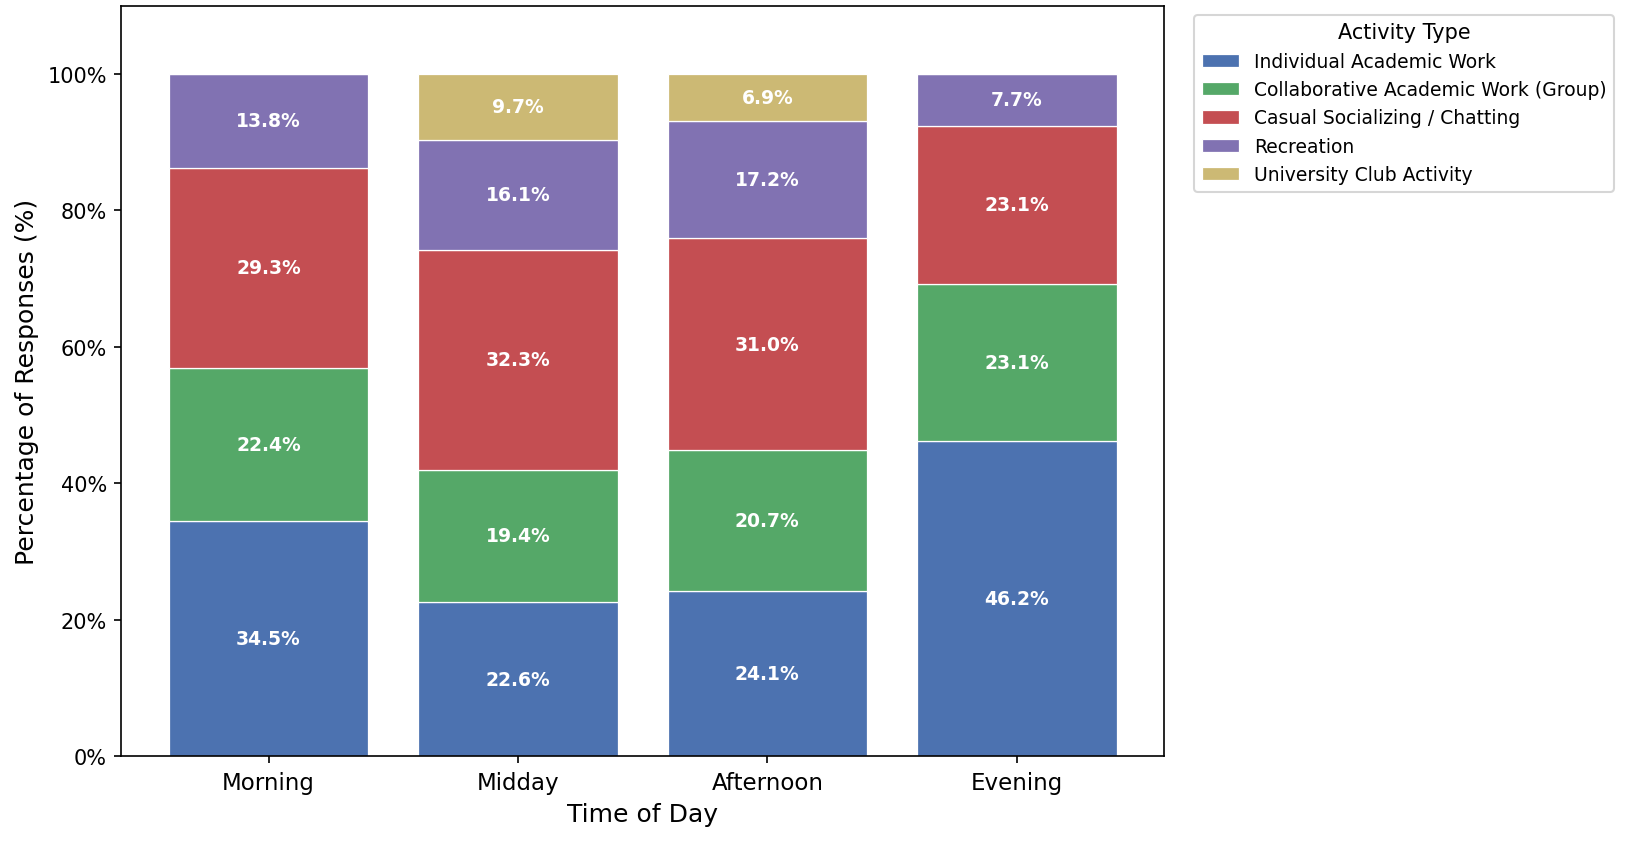
\includegraphics[width=1.1\linewidth]{figures/interval_vs_activity.png}
    \caption{Activities performed in the Open area by time of day}
    \label{fig:Activities}
\end{figure}

\newpage
\section{Association between interval and activity type}

\begin{description}
    \item[H0:] Activity type is independent of time interval.
    \item[H1:] Activity type is associated with time interval.
\end{description}

Five types of activities reported in the survey were coded into two groups – Academic and Non-academic – for the purpose of analysis. This was because in order to conduct a Chi-Square test on the basis of this table, at least one cell in every row and column must have a value greater than five. With 133 respondents spread over four time intervals and five activity categories, some cells of the larger contingency table do not meet this requirement.

\begin{table}[H]
    \centering
    \caption{Observed counts of Academic vs Non-academic activity by interval}
    \label{tab:contingency}
    \begin{tabular}{|l|c|c|}
        \hline
        \textbf{Interval} & \textbf{Academic} & \textbf{Non-academic} \\ \hline
        Morning   & 32 & 17 \\ \hline
        Midday    & 13 & 16 \\ \hline
        Afternoon & 13 & 16 \\ \hline
        Evening   & 18 & 8  \\ \hline
    \end{tabular}
\end{table}

\begin{table}[H]
    \centering
    \caption{Chi-Square test of independence: Interval x Activity Type}
    \label{tab:chisq}
    \begin{tabular}{|l|c|c|c|c|}
        \hline
        \textbf{N} & \textbf{$\chi^2$} & \textbf{df} & \textbf{p-value} & \textbf{Cram\'er's V} \\ \hline
        133 & 6.477 & 3 & 0.091 & 0.221 \\ \hline
    \end{tabular}
\end{table}
The null hypothesis was found to be true for the relationship between time interval and nature of activities since at the $\alpha=0.05$ level of significance, it did not attain statistical significance ($p=0.091$). However, the counts are found to follow the anticipated trend (greater number of academic activities than non-academic activities in the Morning and Evening categories, and vice versa in the Midday and Afternoon intervals), and the small to moderate strength of association (Cram\'er's V = 0.221) points towards a significant association, albeit a weak one.
\chapter{Environmental Stressors \& Displacement}

\section{Diurnal variation in environmental comfort}
First we must identify if there is a significant change in environmental stressors.

\begin{figure}[H]
    \centering
    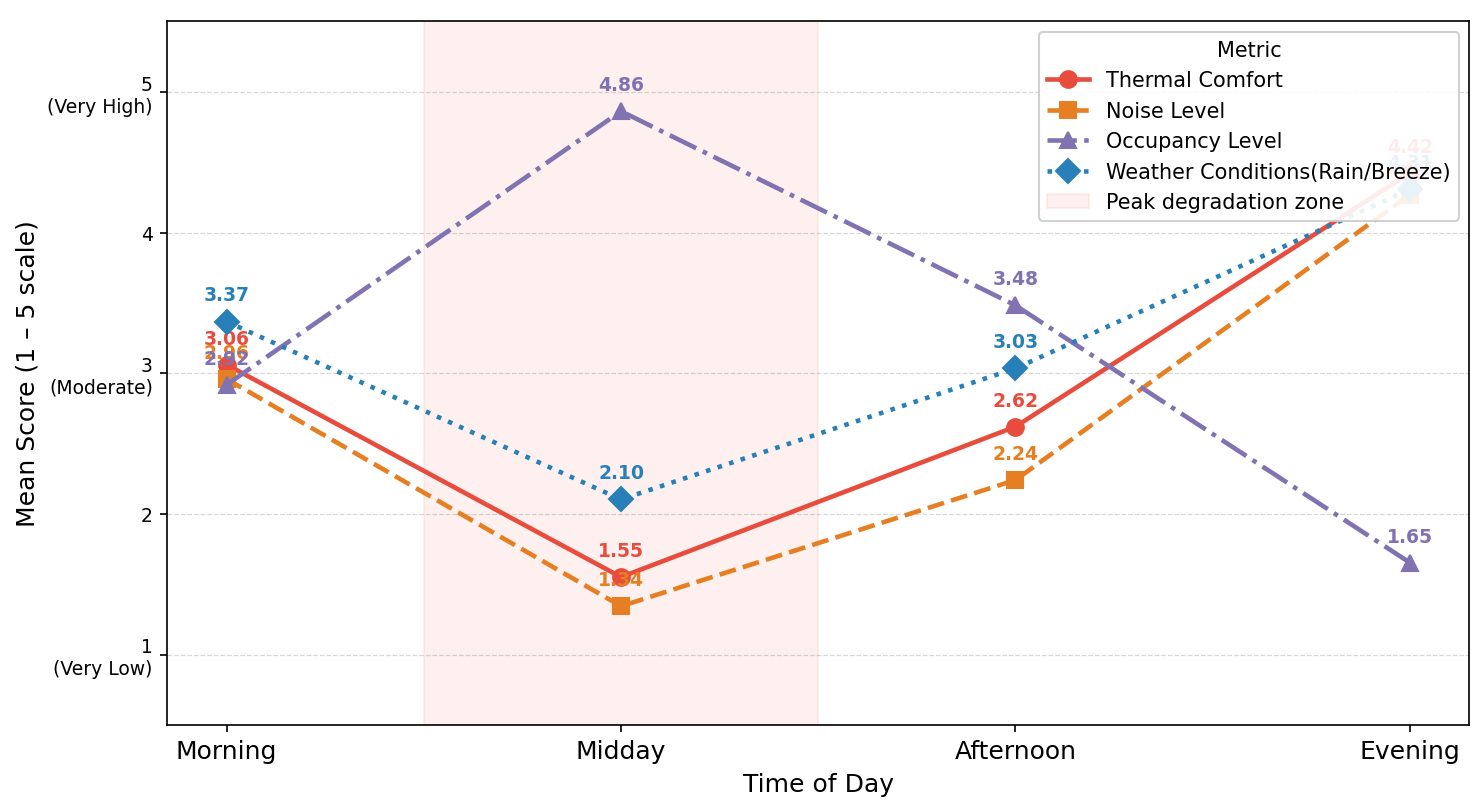
\includegraphics[width=0.9\linewidth]{figures/trend_a_diurnal_degradation.png}
    \caption{Average environmental comfort ratings by time of day}
    \label{fig:diurnal}
\end{figure}

\begin{description}
    \item[H0:] The distribution of environmental comfort ratings is identical across all four diurnal time blocks (i.e. environmental conditions are constant throughout the day).
    \item[H1:] At least one diurnal time block has a significantly different distribution of environmental comfort ratings compared to the others.
\end{description}

\newpage

Thermal Comfort\index{Thermal Comfort} and Occupancy Level\index{Occupancy Level} were tested across the four intervals using the Kruskal-Wallis H-test\index{Kruskal-Wallis test}.
\begin{table}[H]
    \centering
    \caption{Kruskal-Wallis test of environmental ratings across intervals}
    \label{tab:kruskal}
    \begin{tabular}{|l|c|c|c|c|}
        \hline
        \textbf{Variable} & \textbf{H} & \textbf{df} & \textbf{p-value} & \textbf{Significant ($\alpha=0.05$)} \\ \hline
        Thermal Comfort  & 75.662 & 3 & $<0.001$ & Yes \\ \hline
        Occupancy Level  & 82.164 & 3 & $<0.001$ & Yes \\ \hline
    \end{tabular}
\end{table}

However, in both cases, the level of significance is much greater than the $\alpha = 0.05$ level; therefore, we will reject the null hypothesis in both cases, the variable of environmental comfort varies throughout the day. The median value of these variables supports the direction of the effect, the median value of Thermal Comfort is minimal at Midday (median value 2) and maximal in the Evening (median value 4); meanwhile, the median value of Occupancy Level is maximal at Midday (median value 5) and minimal in the Evening (median value 2).

\section{Predicting displacement}

\begin{description}
    \item[H0:] Thermal Comfort, Noise Level\index{Noise Level}, and Occupancy Level do not predict the probability of a student leaving the Open Area under a sudden noise disruption.
    \item[H1:] At least one of Thermal Comfort, Noise Level, or Occupancy Level significantly predicts the probability of leaving.
\end{description}

The dependent variable was coded as binary based on the noise disruption question, where 0 indicates that the student would remain (withstanding the noise or moving into a leisure mode), while 1 indicates that the student would depart the Open Area. These values were then modeled against the three current condition variables using binary logistic regression\index{Logistic regression}. This is the appropriate analysis technique for two reasons: the data is both binary and ordinal and the question asked is predictive. The fitted model is:
\begin{multline}
    \boldsymbol{\mathrm{logit}(p_{\mathrm{leave}}) = 0.848 - 0.997(\mathrm{Thermal\ Comfort})} \\
    \boldsymbol{{}+ 0.528(\mathrm{Noise\ Level}) - 0.048(\mathrm{Occupancy\ Level})}
    \label{eq:logit}
\end{multline}

\begin{table}[H]
    \centering
    \caption{Logistic regression predicting displacement from environmental ratings}
    \label{tab:logit}
    \begin{tabular}{|l|c|c|c|c|}
        \hline
        \textbf{Predictor} & \textbf{Coefficient} & \textbf{Std. Error} & \textbf{p-value} & \textbf{Odds Ratio} \\ \hline
        Intercept        & 0.848  & 1.493 & 0.570 & 2.335 \\ \hline
        Thermal Comfort  & -0.997 & 0.343 & 0.004 & 0.369 \\ \hline
        Noise Level      & 0.528  & 0.404 & 0.190 & 1.696 \\ \hline
        Occupancy Level  & -0.048 & 0.253 & 0.850 & 0.953 \\ \hline
    \end{tabular}
\end{table}

\begin{table}[H]
    \centering
    \caption{Model fit statistics}
    \label{tab:logitfit}
    \begin{tabular}{|c|c|c|}
        \hline
        \textbf{N} & \textbf{Pseudo $R^2$ (McFadden)} & \textbf{LLR p-value} \\ \hline
        133 & 0.078 & 0.0042 \\ \hline
    \end{tabular}
\end{table}

The overall model is statistically significant (LLR $p = 0.0042$), and hence H0 is rejected; the environmental ratings collectively explain the probability of displacement from the Open Area, but the low pseudo $R^2$ suggests other unseen variables contribute to this decision as well. Out of the three variables, only Thermal Comfort is significant ($p = 0.004$); with each unit increase in thermal comfort, there is a 63\% decrease in the probability of being displaced from the Open Area (OR = 0.369). The variables Noise Level and Occupancy Level do not attain statistical significance after controlling for Thermal Comfort. For RQ2, thermal discomfort, but not noise and crowding separately, appears to be the environmental stressor driving students' displacement from the Open Area.

\chapter{Infrastructure \& Tolerance}

\section{Infrastructure as a modulator of tolerance}

\begin{description}
    \item[H0:] Reaction to a noise disruption (stay vs leave) is independent of power dependency.
    \item[H1:] Reaction to a noise disruption is associated with power dependency.
\end{description}

Power Dependency\index{Power Dependency} (No device / Using battery power / Using wall power) was analyzed through cross-tabulation using the same dichotomous variable of stay/leave as in the displacement\index{Displacement} scenario and was subjected to a Chi-Square test of independence\index{Chi-Square test} since the variables are categorical.
\begin{figure}[H]
    \centering
    
\includegraphics[width=\linewidth]{figures/infrastructure_analysis.png}
    \caption{Infrastructure pull factors, power dependency, and fan-installation impact}
    \label{fig:infra}
\end{figure}

\begin{table}[H]
    \centering
    \caption{Reaction to a noise disruption by power dependency}
    \label{tab:power_noise}
    \begin{tabular}{|l|c|c|c|}
        \hline
        \textbf{Power Dependency} & \textbf{Leave} & \textbf{Stay} & \textbf{\% Leave} \\ \hline
        No device        & 5  & 59 & 7.8\%  \\ \hline
        Battery power     & 23 & 9  & 71.9\% \\ \hline
        Plugged into wall socket & 16 & 21 & 43.2\% \\ \hline
    \end{tabular}
\end{table}

\begin{table}[H]
    \centering
    \caption{Chi-Square test: Power Dependency x noise reaction}
    \label{tab:chisq_power}
    \begin{tabular}{|c|c|c|c|}
        \hline
        \textbf{N} & \textbf{$\chi^2$} & \textbf{df} & \textbf{p-value} \\ \hline
        133 & 41.939 & 2 & $<0.001$ \\ \hline
    \end{tabular}
\end{table}

The relationship is very significant ($\chi^2 = 41.939$, $df = 2$, $p < 0.001$, Cram\'er's V = 0.562, large effect size), therefore H0 is rejected, power dependence has an influential impact on disruption tolerance. This pattern does not reflect a mere linear relationship of the form “the more infrastructure you have, the more tolerant you are.” Students who don’t have a device leave least (7.8%), as they do not have any reasons to go anywhere else. Students using the battery power leave most (71.9%), as they have the freedom to leave anywhere without the risk of cutting off their access to power. Students plugged into a wall socket leave somewhere in the middle (43.2%). Being bound to that particular power source, they are more anchored than students on battery power but still leave much more often than those without any devices.

\chapter{Discussion}

\section{Quantitative results against initial findings}
The inferential results provide a more mixed assessment of the qualitative findings than a uniform one. First, the daily comfort profile is supported strongly: both Kruskal-Wallis tests showed that Thermal Comfort and Occupancy Level differ significantly between intervals ($p < 0.001$ for both), consistent with the qualitative finding about Midday being the most uncomfortable and crowded time, the very time at which the D1 session of observation showed students building Vesak lanterns on the desks, and distrupting the ordinary fuctioning of the space. The distinction between academic and non-academic activities during intervals, however, is less clearly supported, the Chi-Square test does not achieve statistical significance ($p = 0.091$), although the counts behave as expected, and the qualitative description of there being a “diurnal” difference, partly based on interviews describing morning as “tranquil” for studies, does not hold up statistically as well as the interviews claimed.Displacement model adds to the qualitative understanding: In the D1 interviews, heat was the most commonly mentioned environmental factor, yet only Thermal Comfort showed up as an important independent predictor of displacement ($p = 0.004$), implying that heat is the more impactful stressor when noise is also included in the equation. Lastly, the Power Dependency theory provided new insight into qualitative results in areas that D1 had not thought of: Device charging was the most common physical factor influencing students' seating position, but what this paper reveals is how this factor influences students via mobility and anchoring, not merely comfort.

\section{Real-world implications}
One thing is true for all tests within this report and that is the importance of thermal comfort. It is the only factor that is significant in both the diurnal comparison and the displacement model. This means that there is evidence-based support for the installation of fans, which D1 and D3 already demanded: fans not only add to comfort but also fight the Midday decrease in academic motivation and noises-induced displacement. The role of the charging infrastructure is different but equally tangible. As seen from the results of the Power Dependency experiment, when being charged, students are anchored in place (43.2\% leave rate) compared to battery-powered students (71.9\%). That is, while charging infrastructure attracts academic users, as D3 found out, it also decreases the chances of displacement.

\section{Task urgency and spatial preference}
As shown by Harrop and Turpin (2013)\index{Harrop and Turpin (2013)}, however, students' spatial preferences on campus do change, depending on task urgency.\index{Task urgency} The deadline behaviour question of this survey probes this hypothesis directly: in case of a tight deadline the following day for their assignment, 54.1\% of the students indicated that they would stay in the Open Area (either to keep working or move to another location because of disruption), whereas 45.9\% indicated that they would leave and go to either library or home. These roughly even proportions are in line with Harrop and Turpin's hypothesis: normally, the Open Area is "good enough" for most of the students, as is reflected in the relatively low leave proportions in case of a social noise disruption, but once task urgency is raised, much higher proportions of students opt for an environment which is more controlled and less disruptive.

\chapter{Critical Analysis}

The research questions have evolved significantly from those first proposed to those found in this report; at first, the questions were very general in nature regarding how the space was used and what influenced usage, but these were too descriptive in nature to be tested statistically and had thus been changed by D4.

The non-significant outcome of the Chi-Square test conducted on interval and type of activity ($p = 0.091$) cannot be interpreted as an invalidation of the diurnal cycle D1 and D3 identified, the disturbance caused to the research due to the Vesak lanterns mentioned above is just one example.

Other limitations exist: The survey uses self-reported intention to behave (like hypothetical questions about deadlines and noise disruption), which may not align with real behavior, and cross-sectional data design only shows association and not the process assumed by the predictive approach.

\chapter{Conclusion and Future Work}

In four stages, this study progressed from simple observation to hypothesis tests on the UCSC Open Area. Thermal comfort emerged as the most stable influence found in both diurnal analysis and the displacement models. Although the marginal interval-activity relation ($p = 0.091$) still requires replication using a bigger, week-long sample including weekends to see whether it holds or represents another confounding factor of the Vesak festival mentioned above. Access to infrastructure influences displacement not by comfort but mobility and anchoring. The qualitative stage did not reveal it as well; causal confirmation could be done using a before-after design with upgraded fans and charging stations, instead of stated preferences only. Task urgency revealed yet again that tolerance of the space is contingent and depends on other factors \citep{harrop2013}. Other D3 relations --- the Afternoon peak for Collaborative Academic Work, lack of lighting causing low Evening use, and connection between duration of session and number of visits,  were not confirmed and remain the topic for future research.

Combining all the evidence, it becomes clear that thermal comfort and good charging facilities are the two strongest aspects of the Open Area that need improvement.



\renewcommand{\bibname}{References}
\addcontentsline{toc}{chapter}{References}
\begin{thebibliography}{99}

\bibitem[Harrop and Turpin, 2013]{harrop2013} Harrop, D. and Turpin, B. (2013) 'A study exploring student behaviours in informal learning spaces', \textit{Higher Education Quarterly}, 67(1), pp.~38--58.

\end{thebibliography}


\printindex

\end{document}